\section{Team Structure}
\label{sec:team}

As in the initial report, we use the following acronyms for team members:

\begin{tabular}{ p{3cm} p{4cm} p{3.5cm} p{3.5cm} }
  \textbf{AJF}-Adam Fahie &
  \textbf{AIF}-Andrew Fairbairn &
  \textbf{TF}-Anthony Free &
  \textbf{TD}-Tom Davies \\
    \textbf{RT}-Rosy Tucker &
  \textbf{JM}-Joseph Mansfield &
  \textbf{MW}-Michael Walker \\
\end{tabular}

Before beginning this stage of the project, we ascertained which university modules team members were studying, in order to spread the work load evenly and reduce the risk of team members' under performance due to other commitments. We also assessed the strengths and weaknesses of each team member, aiding in the selection of technologies and task assignment, as shown in table \ref{tab:skills}. Table \ref{tab:skills} shows that all team members are proficient with Java, and thus it was a natural implementation choice for the prototype.

All team members contributed to the design of the HUMS architecture, however, when implementing the prototype the team divided into three sub-teams, each assigned to different modules and requirements for the system.
The sub-teams were organised such that team members with similar skills and knowledge were placed together, encouraging low coupling and rapid development of individual modules, without worrying about the state of the overall system. The tasks assigned to each sub-team are shown below, reporting and notification engines were not assigned to any particular sub-team, meaning all team members were able to contribute to designs, encouraging creativity.

\begin{description}
  \item[Team Sense  (JM and MW)] Create a data emitter for the test application, by producing reusable monitoring components.and implement the data input API as a multithreaded server, in order to meet requirements  regarding simultaneous usage.
    
  \item[Team Store  (TD and RT)] Implement the database abstraction layer, and provide a concrete implementation using Google App Engine as a backing store, keeping the API generic in order to meet requirements regarding flexibility of database implementation.

  \item[Team Analyse (AJF, AIF, and TF)] Implement the analysis controller and the analysis engine API. The engine API was implemented to be very sparse so that a large number of different concrete implementations could be supplied. 
\end{description}

Other than the introduction of subteams for development, the team organisation
did not change from the first phase, as we found that the previously allocated
roles worked well.

\begin{table}[H]
\centering
\begin{tabular}{|p{1.2cm}|p{8cm}|p{5cm}|}
  \hline \rowcolor{titleColor}\textbf{Initials} &
  \textbf{Experience} &
  \textbf{Weaknesses}\\

  \hline AJF
  & Java, C, Ruby, Spring, Hibernate, Gradle, Design Patterns, Tomcat, JBoss,
  Git, SQL
  & Web Development, NoSQL, UI/UX, Technical Writing \\

  \hline AIF
  & Java, C++, Python, Javascript, PHP, UI/UX, Web Development, NoSQL/SQL
  & Spring, Technical Writing \\
  
  \hline TF
  & PHP, Javascript, Java, VB, C, Linux, MDE Developer, Git, SQL
  & UI/UX, Technical Writing \\

  \hline TD
  & Java, C, Python, Scala, Android, Swing, Machine Learning, SQL
  & NoSQL, Web Development, Git \\

  \hline JM
  & C, C++, Java, Python, UI/UX, Android, Web Development, Git, SQL
  & Hardware, NoSQL \\

  \hline RT
  & Java, C, Objective-C, Javascript, Android, iOS, Swing, Design Patterns,
  Google AppEngine, HCI, NoSQL/SQL, Attribute Driven Design
  & Spring, Git \\

  \hline MW
  & C, Java, Python, Git
  & UI/UX, Technical Writing, Concurrency \\
  \hline
\end{tabular}
\caption{The identified strengths and weaknesses of team members}
\label{tab:skills}
\end{table}

\subsubsection{Time Management}
As a team we considered the scope of the project which was to be undertaken.
 As a result of this we divided the work to be undertaken into specific tasks.
 Once the work to be undertaken was identified, the work was evenly split across 
the three sub-teams, and working as part of our three teams, again split the 
 tasks between us to ensure an equal workload.
 
Dependencies between tasks were extracted, to enable critical path analysis of the project. 
This allowed us to ensure that for each task, the prerequisite task would be completed 
prior to the next task commencing. \hl{The workflow can be seen in the Gantt chart displayed in 
figure XXX, the key for the Gantt chart is displayed in figure YYY.}
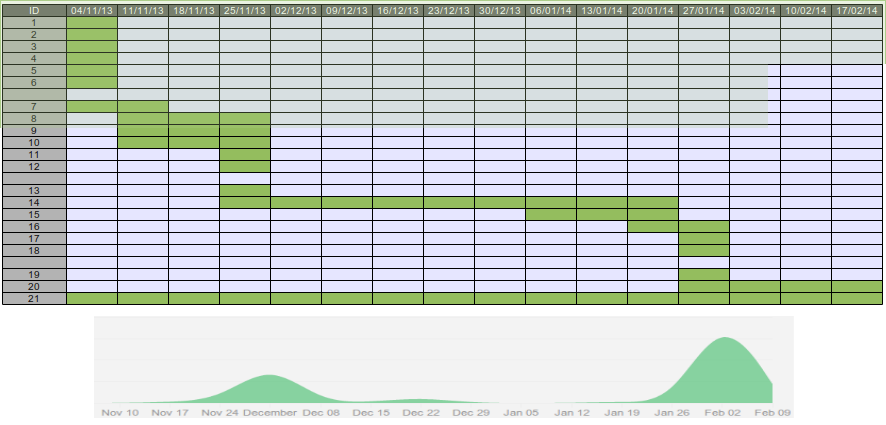
\includegraphics[scale=0.48]{images/GanttChart.png}

\begin{table}[H]
\centering
\begin{tabular}{|p{1.2cm}|p{8cm}|p{5cm}|}

\end{tabular}
\end{table}
